\documentclass[a4paper, 11pt, titlepage]{article}
\usepackage[utf8]{inputenc}
\usepackage{kvoptions-patch}
\usepackage[title={Sistema experto en CLIPS \\ Apoyo a la inversión en bolsa}]{estilo}

\makeatletter
 \renewcommand{\ALG@name}{Pseudocódigo}
\makeatother

\begin{document}

    \maketitle

    \pagenumbering{roman}
    \tableofcontents
    \newpage

    \pagenumbering{arabic}

    \section{Resumen del funcionamiento del sistema}

    El sistema experto desarrollado actúa como un apoyo a la inversión en bolsa. Dada una cartera de valores, el estado actual del mercado y la situación político-económica que se deriva de las noticias de los medios de comunicación de los últimos días, el sistema oferta hasta cinco propuestas diferentes de movimientos de tres tipos: compra de acciones de un valor del que se espera una alta rentabilidad, venta de acciones de un valor de la cartera del que se espera una baja rentabilidad y un intercambio de acciones de un valor de la cartera a otro valor del mercado ---que puede estar o no en la cartera--- para conseguir una mayor rentabilidad.

    El sistema es un apoyo, luego es el usuario el que tiene la última palabra en todas las propuestas: es él quien decide si ejecutar o no una propuesta y qué cantidad de acciones quiere comprar, vender o intercambiar cuando elige llevar a cabo una.

    Además, el sistema permite el almacenamiento de la cartera actual en cualquier momento; así, el resultado de ejecutar cualquier propuesta puede guardarse para días posteriores.

    En la figura \ref{fig:diagrama} se puede ver de forma gráfica el funcionamiento general del sistema, indicando sólo entradas y salidas sin entrar en detallar el funcionamiento interno del sistema.
    \begin{center}
        \begin{figure}[!htb]
            \centering
            \includegraphics[width=\textwidth]{00-DiagramaSistema.png}
            \caption{Diagrama general del sistema.}
            \label{fig:diagrama}
        \end{figure}
    \end{center}


    \section{Proceso seguido en el desarrollo}

    El desarrollo del sistema ha seguido ---a pequeña escala y teniendo en cuenta que experto, directivo y usuarios eran simulados por una misma persona--- el proceso de ingeniería del conocimiento estudiado en las sesiones de teoría: estudio del problema en documentos relevantes, reuniones iniciales con el experto para una primera toma de contacto, reuniones posteriores para delimitar los detalles y contactos con los directivos y usuarios para definir entradas y salidas del sistema.

    Por último, se ha llevado a cabo un proceso de validación y verificación intentando replicar las técnicas vistas en las sesiones de teoría.

    \subsection{Sesiones con el experto}

    En total se produjeron tres reuniones con el experto: una en clase de teoría y dos en clases de prácticas. El conocimiento que faltaba para poder diseñar e implementar el sistema se extrajo del documento \emph{online} proporcionado por el experto.

    En la primera sesión ---la producida en una clase de teoría, y en la que el experto actuó también de directivo y usuario---, se definieron de forma muy general las entradas y salidas del sistema, se indicaron las primeras tareas, como la detección de valores estables o peligrosos y se obtuvo una primera idea del razonamiento que el usuario quería ver cuando se le ofreciera una propuesta. Además, se dieron algunas pinceladas sobre lo que sería el funcionamiento del sistema final, como el apunte de que se mostraran las cinco mejores propuestas calculadas y de dónde había que obtener las variables de entrada.

    En la segunda sesión, ya en una clase de prácticas, se detallaron de forma más precisa los módulos ---los módulos de detección de valores estables e inestables, de valores peligrosos, de valores sobrevalorados, de valores infravalorados y el módulo de gestión de la inversión---, estructura que se ha mantenido hasta el final. En concreto se dio una idea de cómo funcionaría el módulo de detección de valores peligrosos, indicando que las entradas serían los valores de la bolsa durante los últimos 5 días y cómo se han desplazado, las noticias y la cartera de acciones ---podemos ver cómo la estructura de las entradas se mantuvo casi completamente hasta el final--- y las salidas serían los valores peligrosos; además, se indicaron un par de reglas que formarían parte de este módulo.

    En esta misma sesión se empezó además a definir la estructura global del sistema, con un esqueleto vacío que implementara ya la comunicación entre módulos, y se determinaron las estructuras de conocimiento con las que se trabajaría.

    Por último, en la tercera sesión con el experto se definieron algunos conceptos bursátiles que los ingenieros del conocimiento desconocíamos, se dieron nuevas reglas y se discutió acerca de la idoneidad de tener el conocimiento por escrito ---de donde se obtuvo el documento \emph{online} que ha sido clave en el desarrollo del sistema---.

    \subsection{Procedimiento de validación y verificación}

    El proceso de validación y verificación del sistema se ha realizado siguiendo las pautas vistas en las sesiones teóricas, intentando explotar al máximo las técnicas propias de ingeniería del conocimiento sin dejar de lado las técnicas generales de ingeniería del software que en ocasiones se podían aplicar.

    Veamos paso por paso el procedimiento seguido.

    \subsubsection*{Verificación}
    El primer paso de este proceso ha sido la verificación; es decir, la comprobación de que el código implementado era correcto.

    El estudio de la consistencia se ha hecho analizando el comportamiento de las reglas y cómo unas actuaban sobre otras, creando ejemplos ficticios para poder llegar a estados de conflicto. Lo único que se detectó en este caso fue un estado en el que convivían en la base de datos dos hechos del tipo \code{(Modulo $i$)} y \code{(Modulo $j$)}, con $i \neq j$, y se decidió trabajar con un único hecho siempre, que se modifica cuando se quiere cambiar de módulo.

    Por otro lado, en el estudio de la sintaxis se detectó que muchos de los valores de los atributos de las empresas no estaban bien expresados, como en el caso de los valores \code{DISPONIBLE} y \code{GRANDE}, que hasta ese momento se estaban usando en minúscula y hacían que ninguna de las reglas que lo contenían se ejecutara.

    La completitud se analizó comparando el documento \emph{online} dado por el experto con el código, haciendo de nuevo casos de prueba para detectar algún fallo. En esta fase no se detectó nada y, tras un estudio exhaustivo del documento se concluyó que el sistema era completo.

    \subsubsection*{Validación}
    El último paso de este proceso ha sido la validación; es decir, la comprobación de que el código implementado, además de ser correcto, cumple con las necesidades del usuario.

    En un primer momento se ha realizado un proceso de validación objetiva, en el que se ha analizado cada una de las reglas implementadas para asegurarnos de que cumplían con lo dictado por el experto ---en este caso, con lo descrito en el documento \emph{online}---.

    Para llevar a cabo esta tarea se han hecho tests unitarios para comprobar que las reglas cumplían con toda la casuística considerada: se han añadido a la cartera valores ficticios que cumplieran con las hipótesis, otros que no lo hicieran e intentando buscar casos extremos que pudieran hacer ver un mal funcionamiento del sistema, como puede ser el caso de la compra de más acciones de las que podemos pagar o de la venta de un número negativo de acciones. Se ha intentado aquí también estudiar la jerarquía entre las reglas, analizando cuáles se ejecutaban primero y si esto producía algún error. Con esta técnica se pudo comprobar, por ejemplo, que las noticias positivas no tenían más poder que las negativas; esto se cambió convenientemente asignando prioridades a las reglas.

    Además, se ha estudiado la implementación y se ha analizado su modularidad, estudiando la facilidad de mantenimiento y la claridad del código. En esta fase se pulieron muchos detalles, intentando encapsular todo lo posible las reglas y los métodos para que fueran reutilizables y claros.

    Por último, se ha llevado a cabo una validación interpretativa, en la que se ha actuado como usuarios con distintas necesidades para poder pulir la interacción con los mismos ---como no teníamos acceso a los usuarios finales, la valoración de estos aspectos ha sido llevada a cabo por el ingeniero del conocimiento, buscando siempre la máxima facilidad de uso---. Se han buscado así errores que no se vieron en la fase anterior ---de casos muy concretos, como la posibilidad de comprar acciones de un valor que ya teníamos en la cartera--- y modificando pequeños aspectos de usabilidad e interacción.

    \section{Descripción detallada del sistema}

    En esta sección vamos a analizar detenidamente el funcionamiento del sistema, los módulos que lo forman, cómo interactúan entre ellos y las reglas que conforman el razonamiento, teniendo siempre en cuenta que se ha seguido una representación y un razonamiento simbólicos.

    \subsection{Variables de entrada del problema}
    \label{ch:varEntrada}

    El sistema tiene las siguientes variables de entrada:

    \begin{enumerate}
        \item \textbf{Cartera de valores}: Archivo de texto con información sobre la cartera de valores del usuario. Cada línea del archivo se corresponde con un valor en el que el usuario tenga inversión y está compuesta por los siguientes campos, delimitados por espacios:
        \begin{itemize}
            \item Nombre del valor: cadena de caracteres que identifica de forma unívoca un valor.
            \item Número de acciones: cantidad de acciones de esa empresa que tiene el usuario.
            \item Valor: cantidad de dinero que valen las acciones; este número ---en euros--- debe coincidir con el producto \code{número de acciones} $\times$ \code{precio de cada acción}.
        \end{itemize}
        Este archivo debe contener, al menos, una línea con el nombre \code{DISPONIBLE}, que informa de la cantidad de dinero líquido disponible, indicada en el campo \code{Valor}. El campo \code{número de acciones} de esta línea es irrelevante, aunque suele coincidir con el de \code{Valor}.

        \item \textbf{Análisis de los valores del mercado}: Archivo de texto con información sobre el estado actual de  los valores del Ibex35. Cada línea del archivo se corresponde con un valor del Ibex35 y está compuesta por los siguientes campos, delimitados por espacios:
        \begin{itemize}
            \item Nombre: cadena de caracteres que identifica de forma unívoca un valor.
            \item Precio: precio ---en euros--- de una acción.
            \item VarDia: variación del valor con respecto al día anterior ---en tanto por ciento---.
            \item Capitalización: valor total de la empresa ---en miles de euros---.
            \item Ratio precio-beneficio (PER): capitalización dividida por los beneficios anuales obtenidos por la empresa ---en tanto por ciento---.
            \item Rentabilidad por dividendo (RPD): ratio que indica la cantidad recibida por los accionistas por dividendos ---en tanto por uno---.
            \item Tam: cadena de caracteres que indica el tamaño de la empresa: \code{GRANDE}, \code{MEDIANA} o \code{PEQUENIA}.
            \item Ibex: capitalización con respecto al total del Ibex ---en tanto por ciento---.
            \item EtiqPER: cadena de caracteres que indica el estado actual del PER: \code{Alto}, \code{Medio} o \code{Bajo}.
            \item EtiqRPD: cadena de caracteres que indica el estado actual del RPD: \code{Alto}, \code{Medio} o \code{Bajo}.
            \item Sector: cadena de caracterres que identifica de forma unívoca el sector al que pertenece la empresa.
            \item Var5Dias: variación del precio respecto al que tenía hace cinc días ---en tanto por ciento---.
            \item Perd3Consec: valor booleano que indica si la empresa ha tenido pérdidas durante los últimos tres días ---\code{true}--- o no ---\code{false}---.
            \item Perd5Consec: valor booleano que indica si la empresa ha tenido pérdidas durante los últimos cinco días ---\code{true}--- o no ---\code{false}---.
            \item VarRelativaSector: variación de los últimos cinco días relativa a la variación del sector en el mismo tramo temporal ---en tanto por ciento---.
            \item VarRelativaSectorChico: variable booleana que indica si la variación anterior es menor de un -5\% ---\code{true}--- o no ---\code{false}---.
            \item VarMensual: variación del valor con respecto al mes anterior ---en tanto por ciento---.
            \item VarTrimestral: variación del valor con respecto al trimestre anterior ---en tanto por ciento---.
            \item VarSemestral: variación del valor con respecto al semestre anterior ---en tanto por ciento---.
            \item VarAnual: variación del valor con respecto al año anterior ---en tanto por ciento---.
        \end{itemize}

        \item \textbf{Análisis de los sectores del mercado}: Archivo de texto con información sobre el estado actual de los sectores del Ibex35. Cada línea del archivo se corresponde con un sector del Ibex35 y está compuesta por los siguientes campos, delimitados por espacios:
        \begin{itemize}
            \item Nombre: cadena de caracteres que identifica de forma unívoca un valor.
            \item VarDia: variación del valor con respecto al día anterior ---en tanto por ciento---.
            \item Capitalización: valor total de la empresa ---en miles de euros---.
            \item Ratio precio-beneficio (PER): capitalización dividida por los beneficios anuales obtenidos por la empresa ---en tanto por ciento---.
            \item Rentabilidad por dividendo (RPD): ratio que indica la cantidad recibida por los accionistas por dividendos ---en tanto por uno---.
            \item Ibex: capitalización con respecto al total del Ibex ---en tanto por ciento---.
            \item Var5Dias: variación del precio respecto al que tenía hace cinc días ---en tanto por ciento---.
            \item Perd3Consec: valor booleano que indica si la empresa ha tenido pérdidas durante los últimos tres días ---\code{true}--- o no ---\code{false}---.
            \item Perd5Consec: valor booleano que indica si la empresa ha tenido pérdidas durante los últimos cinco días ---\code{true}--- o no ---\code{false}---.
            \item VarMensual: variación del valor con respecto al mes anterior ---en tanto por ciento---.
            \item VarTrimestral: variación del valor con respecto al trimestre anterior ---en tanto por ciento---.
            \item VarSemestral: variación del valor con respecto al semestre anterior ---en tanto por ciento---.
            \item VarAnual: variación del valor con respecto al año anterior ---en tanto por ciento---.
        \end{itemize}
        \item \textbf{Análisis de la situación político-económica}: archivo de texto con información sobre las noticias relevantes al mercado. Cada línea del archivo se corresponde con una noticia y está compuesta por los siguientes campos, delimitados por espacios:
        \begin{itemize}
            \item Nombre: cadena de caracteres que indica el valor del Ibex35 al que hace referencia la noticia ---si la noticia es de carácter general sobre el estado de la economía, este campo contiene la cadena \code{ECONOMIA}---.
            \item Valoración: cadena de caracteres que indica la valoración que hace la noticia sobre la empresa a la que hace referencia; puede ser \code{Buena} o \code{Mala}.
            \item Antigüedad: número de días transcurridos desde la publicación de la noticia.
        \end{itemize}
    \end{enumerate}

    \subsection{Variables de salida del problema}
    \label{ch:defPropuestas}

    El sistema produce un único tipo de salida: una serie de cinco transacciones propuestas, ordenadas de mayor a menor rentabilidad esperada. Cada propuesta se compone de los siguientes apartados:
    \begin{itemize}
        \item Acción de la propuesta: aquí se indica qué se propone ---comprar, vender o intercambiar--- y cuáles son las empresas involuncradas en la transacción.
        \item Rentabilidad esperada: porcentaje de rentabilidad esperada tras ejecutar la transacción propuesta.
        \item Razón: se da un razonamiento exhaustivo de por qué se hace la propuesta, en qué se basa la catalogación de los valores y qué hechos han llevado al sistema a proponer la transacción.
    \end{itemize}

    Además, el sistema es capaz de simular la ejecución de las propuestas elegidas por el usuario y guardar en un fichero de texto, si el usuario así lo desea y con el formato indicado en el primer punto de la sección \ref{ch:varEntrada}, el estado de la cartera tras aplicar las propuestas.

    \subsection{Conocimiento global del sistema}

    La carga de hechos iniciales, definiciones globales y lectura de datos se realiza en el llamado \code{Módulo 0}.

    Allí se define la estructura de la base de conocimiento, declarando plantillas para los valores del mercado y los sectores, para los valores de la cartera, para las noticias y para las propuestas generadas por el sistema.

    Además, se define una variable global usada más tarde en el razonamiento: el precio del dinero, que es el tipo de interés fijado por el Banco Central Europeo para el préstamo de dinero a las entidades financieras; el 10 de marzo de 2016 este tipo de interés se fijó al 0\%. \footnote{Ver http://es.euribor-rates.eu/tipo-de-interes-del-BCE.asp}

    Por último, se genera la base de conocimiento inicial leyendo los ficheros especificados en la sección \ref{ch:varEntrada}, cuyo formato se supone correcto.

    Para más información sobre este módulo inicial, ver la sección \ref{ch:modLectura}.

    \subsection{Especificación de los módulos}

    Definimos aquí el objetivo, conocimiento utilizado y conocimiento deducido de cada uno de los módulos que componen el sistema. Para tener una idea general, resumimos a continuación la lista de módulos:

    \begin{itemize}
        \item Módulo de lectura y detección de valores inestables.
        \item Módulo de detección de valores sobrevalorados.
        \item Módulo de detección de valores infravalorados.
        \item Módulo de obtención de propuestas.
        \item Módulo de interacción con el usuario.
    \end{itemize}

    Además, es necesario explicar de antemano la técnica de gestión de módulos usada de forma unificada por todo el sistema:

    Que una regla pertenezca al módulo $i$-ésimo se caracteriza porque tiene, entre los hechos de sus hipótesis, el hecho \code{(Modulo $i$)}.

    Para avanzar al siguiente módulo, cada uno de ellos tiene definida una regla ---con una prioridad menor que todas las de ese módulo para que se ejecute la última--- que modifica el hecho \code{(Modulo $i$)} y lo actualiza a \code{(Modulo $i+1$)}.

    Al inicio del programa basta añadir el hecho \code{(Modulo 0)} para que todo el razonamiento sea ejecutado desde el principio.

    \subsubsection{Módulo de lectura y detección de valores inestables}
    \label{ch:modLectura}

    Este primer módulo, implementado en los archivos \code{0-EstructuraConocimiento.clp}, \code{0-Lectura.clp} y \code{0-ValoresInestables.clp}, tiene como objetivo la creación de la base de conocimiento inicial a partir de las variables de entrada, generando la estructura para albergar los hechos iniciales, leyendo la información que conformará esos hechos y haciendo el primer razonamiento del sistema: los valores inestables.

    \subsubsection*{Estructura del conocimiento}

    En \code{0-EstructuraConocimiento.clp} se definen plantillas para cada una de las variables de entrada especificadas en la sección \ref{ch:varEntrada}; además de los campos especificados allí, se añaden los siguientes:
    \begin{itemize}
        \item En la plantilla para los valores se añaden tres campos más:
        \begin{itemize}
            \item Rendimiento por año (RPA): el rendimiento por año es, según el experto, la rentabilidad por dividendo más la variación del valor en el último tramo temporal considerado, que se usa como predicción de la variación anual próxima del valor. Hemos considerado aquí como último tramo temporal el último trimestre; el experto apuntó que no debíamos tomar valores muy lejanos, que no permiten tener en cuenta el comporamiento actual del valor, ni demasiado cercanos, que centran el cálculo sólo en un comportamiento muy reciente que no tiene por qué reflejar el comportamiento general. Este valor se mide en tanto por ciento.
            \item Estabilidad: indica si el valor es estable, inestable o no tiene una valoración de la estabilidad especial. Puede tomar los valores \code{NULL} ---este es el valor por defecto---, \code{Estable} e \code{Inestable}.
            \item Valoración: Indica si el valor está sobrevalorado, infravalorado o no tiene una valoración especial; además, se acompaña de una explicación de la valoración actual. Puede tomar los valores \code{NULL} ---este es el valor por defecto---, \code{Sobrevalorado} e \code{Infravalorado}; el razonamiento es una cadena de caracteres.
        \end{itemize}
        \item En la plantilla para los valores de la cartera se añade un campo más:
        \begin{itemize}
            \item Peligroso: indica si el valor es o no peligroso; además, contiene una cadena de caracteres que indica la razón por la que se ha marcado como peligroso. Sus valores pueden ser \code{false} y \code{true}.
        \end{itemize}
    \end{itemize}
    En este primer archivo, como se indicó antes, se define como variable global el precio del dinero.

    \subsubsection*{Lectura de los datos de entrada}

    El archivo \code{0-Lectura.clp} se encarga de leer los archivos de texto de entrada especificados en la sección \ref{ch:varEntrada}.

    Se definen primero una serie de hechos que indican la ruta ---relativa o absoluta--- de los archivos de texto que contienen toda la información. Para poder almacenar la información como hechos, hay definidas reglas para abrir, leer y cerrar los distintos archivos declarados, de manera que una vez ejecutadas la base de conocimiento contiene la información listada en los archivos de texto.

    Además se define una regla para calcular el RPA, tal y como viene indicado en el punto anterior.

    \subsubsection*{Detección de valores estables o inestables}

    El archivo \code{0-ValoresInestables.clp} define las reglas necesarias para detectar valores estables o inestables. Son las siguientes:

    \begin{regla}
        Si un valor $V$ pertenece al sector de la construcción, entonces $V$ es inestable.
    \end{regla}

    \begin{regla}
        Si la economía está bajando ---el Ibex tiene pérdidas en los cinco últimos días--- y un valor $V$ pertenece al sector servicios, entonces $V$ es inestable.
    \end{regla}

    \begin{regla}
        Si hay una noticia positiva sobre un valor $V$ o su sector y la noticia tiene menos de dos días de antigüedad, entonces $V$ es estable.
    \end{regla}

    \begin{regla}
        Si hay una noticia negativa sobre un valor $V$, sobre su sector o sobre la economía en general y la noticia tiene menos de dos días de antigüedad, entonces $V$ es inestable.
    \end{regla}

    Esta serie de reglas definen así la primera parte del razonamiento del sistema: dadas las variables de entrada ---en particular se hace uso de los hechos referentes a valores, a sectores y a noticias---, se obtienen como salida los valores estables o inestables del mercado ---modificando el campo \code{Estabilidad} en los hechos de los respectivos valores---.

    \subsubsection{Módulo de valores sobrevalorados}

    Este módulo tiene como objetivo detectar los valores sobrevalorados del mercado.

    Tiene como única entrada la lista de valores del mercado y, como salida, la misma lista de valores, con el campo \code{Valoracion} marcado como \code{Sobrevalorado} en aquellos valores que lo sean y acompañado del razonamiento usado para marcarlos de tal modo. Las reglas son las siguientes:

    \begin{regla}
        Dado un valor $V$, si su PER está marcado como \code{Alto} y su RPD como \code{Bajo}, entonces $V$ está sobrevalorado.
    \end{regla}

    \begin{regla}
        Dado un valor $V$ cuyo tamaño sea \code{PEQUENIA}:
        \begin{itemize}
            \item Si su PER está marcado como \code{Alto}, entonces $V$ está sobrevalorado.
            \item Si su PER está marcado como \code{Medio} y su RPD como \code{Bajo}, entonces $V$ está sobrevalorado.
        \end{itemize}
    \end{regla}

    \begin{regla}
        Dado un valor $V$ cuyo tamaño sea \code{GRANDE}:
        \begin{itemize}
            \item Si su RPD está marcado como \code{Bajo} y su PER como \code{Medio} o \code{Alto}, entonces $V$ está sobrevalorado.
            \item Si su RPD está marcado como \code{Medio} y su PER como \code{Alto}, entonces $V$ está sobrevalorado.
        \end{itemize}
    \end{regla}

    \subsubsection{Módulo de valores infravalorados}

    Este módulo tiene como objetivo detectar los valores infravalorados del mercado.

    Tiene como única entrada la lista de valores del mercado y, como salida, la misma lista de valores, con el campo \code{Valoracion} marcado como \code{Infravalorado} en aquellos valores que lo sean y acompañado del razonamiento usado para marcarlos de tal modo. Las reglas son las siguientes:

    \begin{regla}
        Si un valor $V$ tiene el PER marcado como \code{Bajo} y el RPD como \code{Alto}, entonces $V$ está infravalorado.
    \end{regla}

    \begin{regla}
        Si un valor $V$ tiene el PER marcado como \code{Bajo}, ha tenido una caída de más de un 30\% en los últimos 3, 6 o 12 meses y ha subido entre un 0\% y un 10\% en el último mes, entonces $V$ está infravalorado.
    \end{regla}

    \begin{regla}
        Si un valor $V$ tiene un tamaño \code{GRANDE}, su RPD está marcado como \code{Alto} y su PER como \code{Medio}, su variación mensual es mayor o igual al 0\% y tiene una variación respecto del sector positiva, entonces $V$ está infravalorado.
    \end{regla}

    Este módulo termina la primera parte del razonamiento del sistema, consistente en razonar sobre la peligrosidad, estabilidad y valoración de cada valor del mercado. Esto conforma la base de conocimiento necesaria para poder generar las propuestas, cuya gestión se hace en el módulo siguiente.

    \subsubsection{Módulo de obtención de propuestas}

    Este módulo tiene como objetivo obtener propuestas para poder ofrecérselas posteriormente al usuario.

    Tiene como entrada toda la base de conocimiento generada en los módulos anteriores ---en particular, usa los hechos relativos a los valores del mercado, a los sectores y a los valores de la cartera, con especial atención a los campos de peligrosidad, estabilidad y valoración--- y, como salida, una serie de hechos del tipo \code{Propuesta} con el formato especificado en la sección \ref{ch:defPropuestas}.

    Las reglas que lo componen son las siguientes\footnote{Todos los valores $PER$, $PER_{sector}$ y $RPD$ que aparece en las reglas están en tanto por ciento.}:

    \begin{regla}
        Si un valor $V$ de la cartera actual es peligroso, en el último mes ha tenido pérdidas, y en ese mismo tramo temporal su caída con respecto a la de su sector es de más de un 3\%, entonces se debe proponer vender las acciones de $V$.

        La rentabilidad esperada de esta propuesta es:
        \[
        RE = 20 - RPD
        \]
    \end{regla}

    \begin{regla}
        Si un valor $V$ está infravalorado y el usuario tiene dinero para comprar al menos una acción de $V$, entonces se debe proponer comprar acciones de $V$.

        La rentabilidad esperada de esta propuesta es:
        \[
        RE = 100 \frac{PER_{sector} - PER}{5 PER + RPD}
        \]
        donde $PER_{sector}$ es el $PER$ del sector al que pertenece $V$.
    \end{regla}

    \begin{regla}
        Si un valor $V$ de la cartera actual está sobrevalorado y su RPA es menor que $5 + PrecioDinero$, entonces se debe proponer vender las acciones de $V$.

        La rentabilidad esperada de esta propuesta es:
        \[
        RE = \frac{PER - PER_{sector} - RPD}{5 PER}
        \]
        donde $PER_{sector}$ es el $PER$ del sector al que pertenece $V$.
    \end{regla}

    \begin{regla}
        Si un valor $V_1$ no está sobrevalorado, un valor $V_2$ de la cartera actual no está infravalorado y el $RPD_1$ de $V_1$ es mayor que la suma $RPA_2 + RPD_2 + 1$ ---donde $RPA_2$ y $RPD_2$ son los campos relativos al valor $V_2$---, entonces se debe proponer cambiar las acciones de $V_2$ por acciones de $V_1$.

        La rentabilidad esperada de esta propuesta es:
        \[
        RE = RPD_1 - (RPA_2 + RPD_2 + 1)
        \]
    \end{regla}

    Cada una de estas reglas, además de deducir el tipo de propuesta y la rentabilidad esperada de cada una de ellas, añaden a la base de conocimiento el razonamiento de por qué se oferta tal propuesta.

    \subsubsection{Módulo de interacción con el usuario}

    Este módulo se encarga de interactuar con el usuario, mostrarle las cinco mejores propuestas actuales y ejecutarlas si fuera necesario.

    Tiene una estructura muy diferente a los módulos anteriores, aunque a grandes rasgos podemos describirlo como sigue:

    Como entradas tiene la interacción con el usuario a través del menú y la base de conocimiento deducida en los módulos previos ---en particular usa hechos relativos a los valores del mercado, a los valores de la cartera y a las propuestas deducidas en el módulo inmediatamente anterior---; como salida incluye la interacción con el usuario, la modificación de la cartera y el almacenamiento de la cartera actual en un archivo en disco.

    El funcionamiento del módulo se rige por el menú, y se comporta de forma general como sigue:

    \begin{enumerate}[I.]
        \item Se imprime un menú por pantalla, dejando al usuario elegir entre varias opciones:
        \begin{enumerate}[1 ---]
            \item Ver estado actual de la cartera: Para cada valor en la cartera, se imprime el número de acciones que posee el usuario y su valor. Se vuelve al paso I.
            \item Ver nuevas propuestas de movimientos: Se imprimen las cinco mejores propuestas calculadas y se deja al usuario ejecutar alguna de ellas. Si no quiere ejecutar ninguna, se vuelve al paso I. Si decide ejecutar alguna, se solicita la información pertinente sobre la propuesta, se ejecuta, se eliminan todas las propuestas y se vuelven a ejecutar los módulos 1, 2, 3 y 4.
            \item Guardar la cartera actual: Actualiza el archivo de texto de donde se leyeron los valores de la cartera volcando los valores de la cartera actual. Se vuelve al paso I.
            \item Salir del programa: Sale del entorno de CLIPS, preguntando antes al usuario si quiere guardar la cartera actual.
        \end{enumerate}
    \end{enumerate}

    Las opciones 1, 3 y 4 son claras; la opción 2, que es quizás la más importante, requiere un poco más de atención, así que la explicamos con detalle:

    Obtenidas todas las propuestas calculadas en el módulo 4, el elegir esta opción hace que el sistema calcule las cinco mejores y se las muestre al usuario. Si el usuario elige alguna de ellas, ocurre lo siguiente:
    \begin{enumerate}
        \item Se solicita al usuario el número de acciones a comprar/vender/cambiar. En el caso del cambio, se solicita sólo el número de acciones a vender del peor valor, mientras que el cálculo de acciones a comprar del valor mejor se hace automáticamente, teniendo en cuenta los precios de ambos valores y manejando la posibilidad de que en la transacción sobre dinero líquido que haya que destinar al valor \code{DISPONIBLE}.

        Además, se gestiona que el número de acciones introducido sea correcto: en el caso de la compra, se comprueba que no sea mayor que el número máximo de acciones que el usuario puede comprar con el dinero disponible; en el caso de la venta o del cambio, se comprueba que no sea mayor que el número máximo de acciones que el usuario ya tiene.
        \item Se ejecuta la propuesta automáticamente, actualizando los valores de la cartera convenientemente.

        \item Como el estado de la cartera ha cambiado, es necesario recalcular los atributos especiales de los valores y obtener nuevas propuestas, por tanto:
        \begin{enumerate}[3.1.]
            \item Se eliminan todas las propuestas actuales.
            \item Se recalculan los atributos especiales de los valores, regresando al módulo 1 con la técnica explicada en la introducción de esta sección.
        \end{enumerate}
    \end{enumerate}

    Con respecto a la implementación de este módulo, es importante destacar que se ha encapsulado el trabajo de la compra y venta de acciones en sendas funciones ---\code{(comprarAcciones)} y \code{(venderAcciones)}---, que se llaman desde las reglas de ejecución de propuesta cuando es necesario; si la propuesta a ejecutar es relativa a un cambio de acciones, se llama a ambas funciones.

    Asimismo, la funcionalidad de obtener las mejores cinco propuestas se ha encapsulado en la función \code{(calcularMejoresPropuestas)}.

    El uso de funciones junto con las reglas ha facilitado la implementación y sencillez del módulo, separando de forma lógica la interacción con el usuario de la ejecución de las propuestas elegidas por este.

    \section{Manual de uso del sistema}

    El archivo \code{InversionBolsa.clp} es el clave para ejecutar el sistema. Desde él se cargan todos los módulos y se añade el hecho \code{(Modulo 0)}.\footnote{La estructura de este archivo está tomada de la práctica de mi compañero Jacinto Carrasco.} Así, para ejecutar el sistema sólo hay que abrir una terminal en el directorio donde se encuentran todos los archivos y ejecutar la siguiente orden:
    \begin{center}
        \code{clips -f InversionBolsa.clp}
    \end{center}

    Antes de comenzar, el usuario puede indicar la ruta de los archivos de texto de entrada al sistema modificando los hechos declarados al principio del archivo \code{0-Lectura.clp}. Modificando las cadenas de texto que se ven en la figura \ref{fig:archivos}, el sistema tomará esos datos como entrada.
    \begin{center}
        \begin{figure}[!htb]
            \centering
            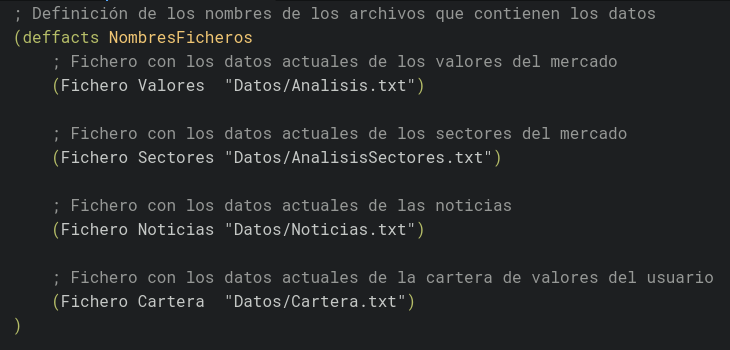
\includegraphics[width=0.7\textwidth]{07-ArchivosTexto.png}
            \caption{Hechos que definen la ruta a los archivos de texto de entrada.}
            \label{fig:archivos}
        \end{figure}
    \end{center}
    Una vez en el sistema, el usuario verá un menú, ---véase figura \ref{fig:menu}---. En este punto se le solicitará qué opción quiere elegir. Veremos cada una de ellas en las siguientes secciones.
    \begin{center}
        \begin{figure}[!htb]
            \centering
            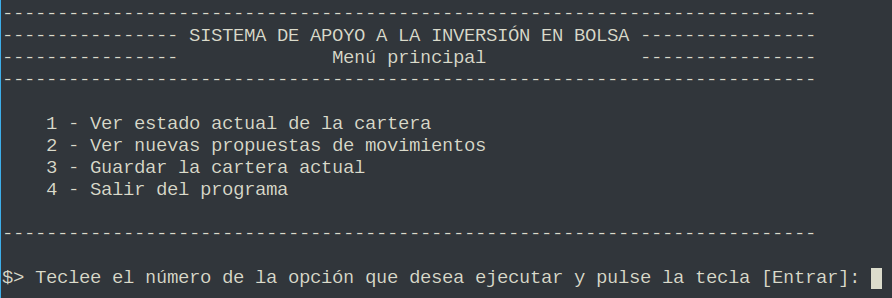
\includegraphics[width=0.8\textwidth]{01-MenuPrincipal.png}
            \caption{Menú principal.}
            \label{fig:menu}
        \end{figure}
    \end{center}

    \subsection{Estado actual de la cartera}

    Si el usuario elige la primera opción, simplemente se le mostrará una pantalla como la que se ve en la figura \ref{fig:cartera}. Para facilitar la visualización de la cartera, el sistema no muestra de nuevo el menú hasta que el usuario no pulsa otra vez la tecla \code{[Entrar]}.

    \begin{center}
        \begin{figure}[!htb]
            \centering
            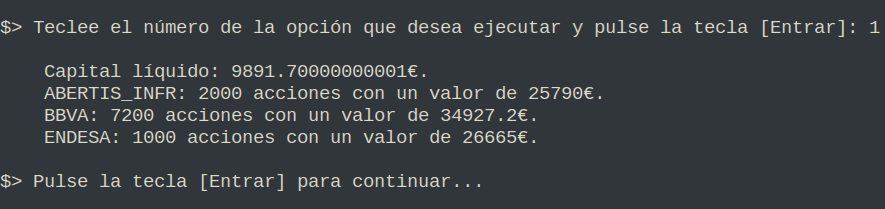
\includegraphics[width=\textwidth]{02-Cartera.png}
            \caption{Cartera de valores.}
            \label{fig:cartera}
        \end{figure}
    \end{center}


    \subsection{Propuestas de movimientos}

    Si el usuario elige la segunda opción, se imprimirán de una vez las cinco mejores propuestas obtenidas por el sistema experto. En la figura \ref{fig:propuestas} se puede ver un ejemplo de dos propuestas distintas, con la transacción que se propone, la rentabilidad esperada y la razón por la que se oferta.

    \begin{center}
        \begin{figure}[!htb]
            \centering
            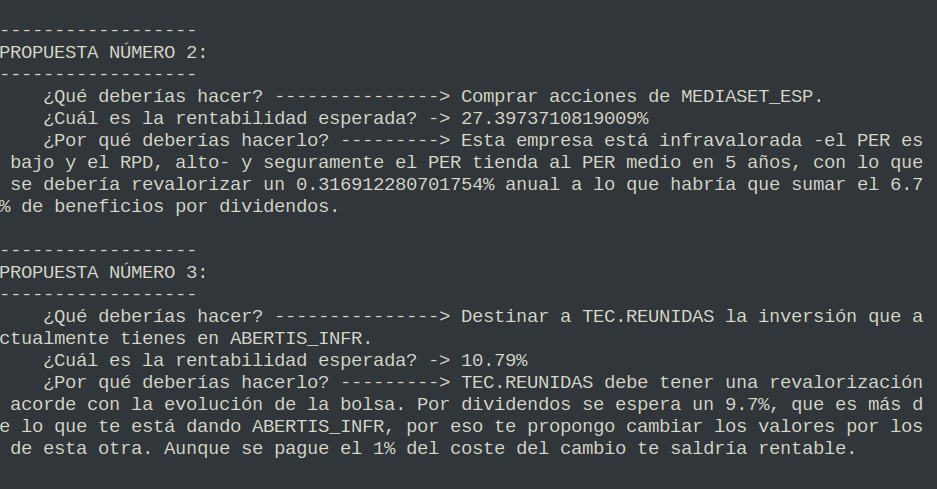
\includegraphics[width=\textwidth]{04-Propuestas.png}
            \caption{Ejemplo de transacciones propuestas al usuario.}
            \label{fig:propuestas}
        \end{figure}
    \end{center}

    Si se decide ejecutar una acción, se solicitará al usuario la información necesaria para llevarla a cabo; a saber: el número de acciones. La figura \ref{fig:ejecucion} muestra la ejecución de la propuesta número 3 vista en la figura \ref{fig:propuestas}, donde se puede ver la interacción entre el sistema y el usuario.

    \begin{center}
        \begin{figure}[!htb]
            \centering
            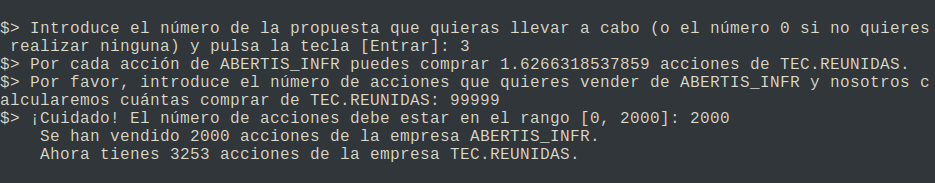
\includegraphics[width=\textwidth]{05-Ejecucion.png}
            \caption{Ejecución de una propuesta de cambio.}
            \label{fig:ejecucion}
        \end{figure}
    \end{center}



    \subsection{Actualización de la cartera en disco}

    Para almacenar los cambios realizados actualizando el archivo en disco, el usuario puede elegir la opción 3. El sistema simplemente actualizará el archivo de texto con el estado actual de la cartera e informará al usuario de que todo ha ido bien. La figura \ref{fig:guardar} da una idea del proceso seguido.

    \begin{center}
        \begin{figure}[!htb]
            \centering
            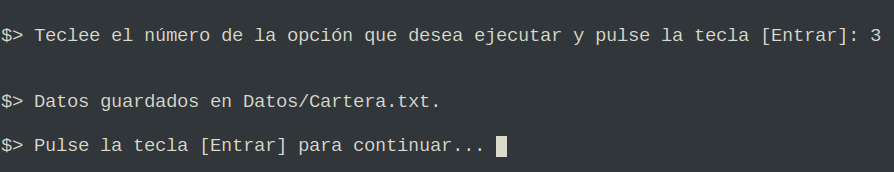
\includegraphics[width=\textwidth]{03-Guardar.png}
            \caption{Actualización en disco de los cambios producidos.}
            \label{fig:guardar}
        \end{figure}
    \end{center}


    \subsection{Terminar el sistema}

    Por último, si se ejecuta la opción número 4, el sistema preguntará si se quiere actualizar el archivo en disco con el estado actual de la cartera. Si el usuario introduce la letra \code{s}, se guardará como en el apartado anterior y se saldrá; si se introduce la letra \code{n}, se saldrá sin guardar; en cualquier otro caso, se volverá a preguntar al usuario para que introduzca una opción correcta. En la figura \ref{fig:salir} se ve un caso de uso de esta opción.

    \begin{center}
        \begin{figure}[!htb]
            \centering
            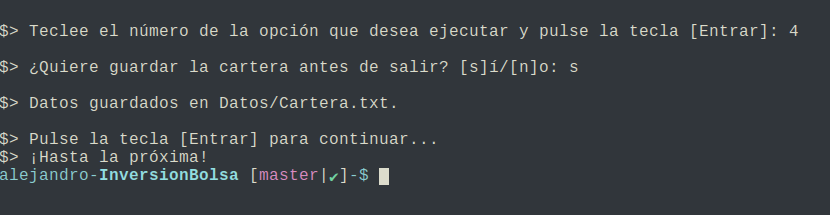
\includegraphics[width=\textwidth]{06-Salir.png}
            \caption{Salir del sistema.}
            \label{fig:salir}
        \end{figure}
    \end{center}


\end{document}
